\subsection{Signal Conditioning}

The process of converting the voltage seen at the current transducer to a digital reading involves three stages (figure \ref{fig:conditioning}).
The gain stage amplifies the voltage of the signal up to a reasonable level.
The filtering stage removes any high frequency noise.
Finally, the sampling stage performs the analog to digital (ADC) conversion.
\begin{figure}[H]
	\centering
	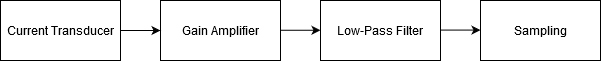
\includegraphics[width=\textwidth]{conditioning}
	\caption{The signal conditioning process.}
	\label{fig:conditioning}
\end{figure}

\subsubsection{Gain Stage}

The current transducers output a $\pm \SI{25}{\milli\volt}$ signal centered around $\SI{2.5}{\volt}$.
This signal must be amplified to $\pm \SI{2.5}{\volt}$ using an operational amplifier with a gain of 100.
To amplify the signal, a non-inverting op-amp circuit (figure \ref{fig:non-inverting-op-amp}) was used.
12 of these circuits are required for each daughterboard.
The LMV324 was selected as it has four op-amp circuits in one package.
Resistor values of $R_1 = \SI{100}{\kilo\ohm}, R_2 = \SI{1}{\kilo\ohm}, R_3 = \SI{10}{\ohm}$ were chosen to give a gain of $100$ and an input impedance of $\SI{1}{\kilo\ohm}$ for each amplifier circuit.

The half-rail voltage of $\SI{2.5}{\volt}$ is provided by a virtual ground op-amp circuit (figure \ref{fig:half-supply}).
An LMV321 was used for this circuit.
High value resistors are required in the divider (typically $\SI{100}{\kilo\ohm}$ to prevent excessive static current drain.
However, these produce greater thermal noise (especially at high ambient temperatures) which is undesirable for ADC applications.
Therefore, two $\SI{2.5}{\kilo\ohm}$ resistors balance the noise and have a static current drain of $\SI{1}{\milli\ampere}$.

\begin{figure}[hb]
\centering

\begin{subfigure}[c]{0.45\textwidth}
	\centering
	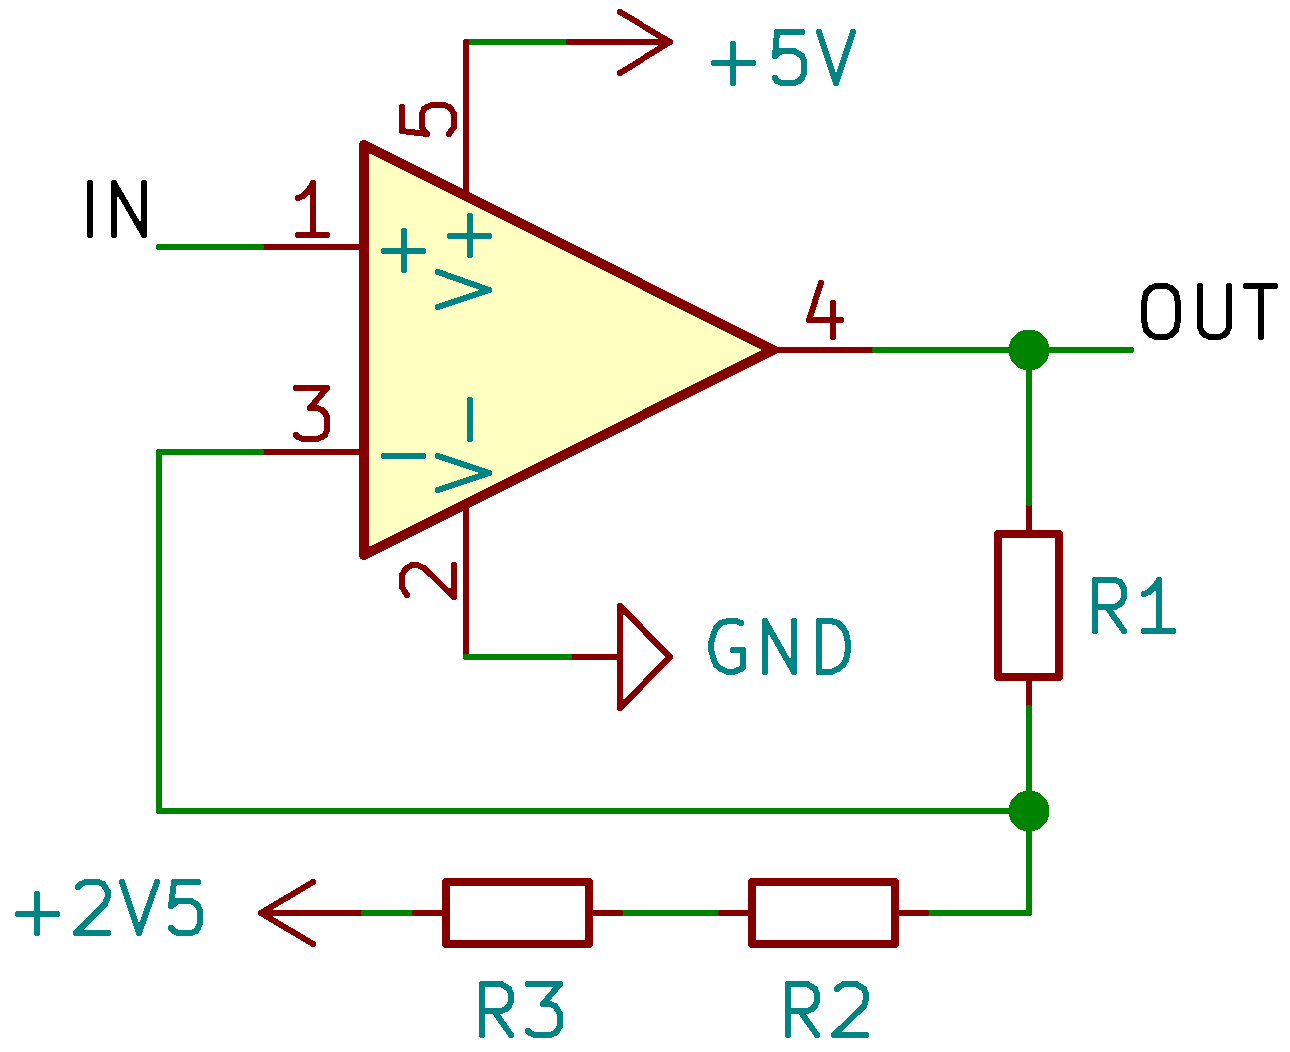
\includegraphics[width=\textwidth]{gain_circuit}
	\caption{The non-inverting amplifier circuit.}
	\label{fig:non-inverting-op-amp}
\end{subfigure}
\hfill
\begin{subfigure}[c]{0.45\textwidth}
	\centering
	\vfill
	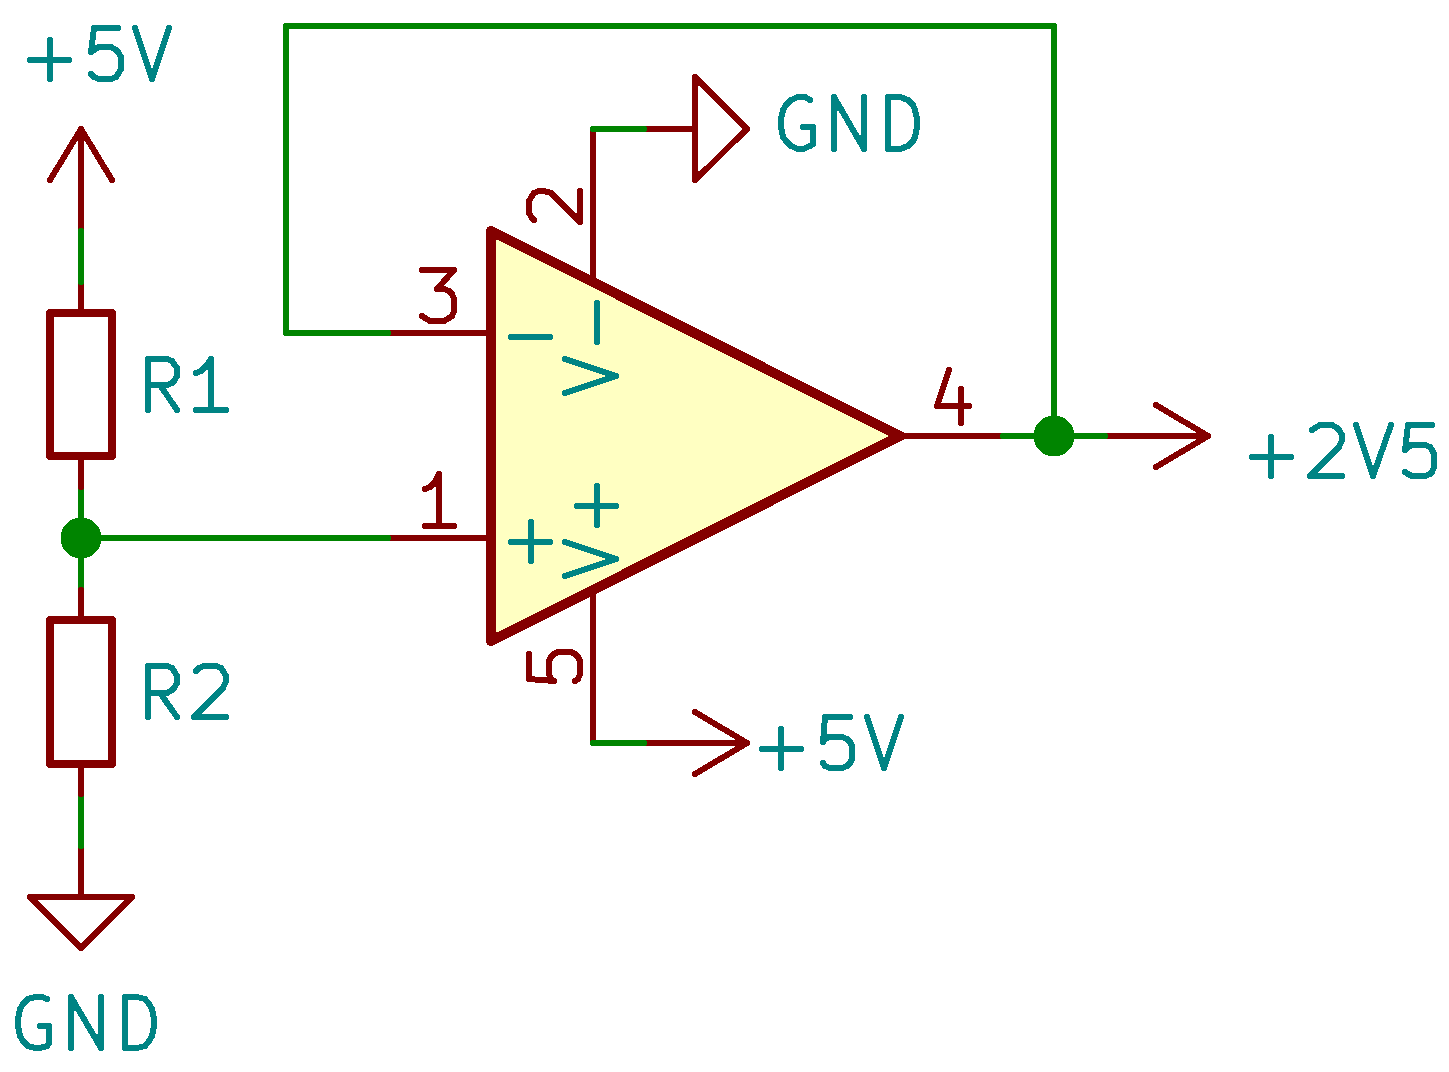
\includegraphics[width=\textwidth]{virtual_ground_circuit}
	\vfill
	\caption{The virtual ground circuit.}
	\label{fig:half-supply}
\end{subfigure}

\caption{The operational amplifer circuits used.}
\end{figure}

The op-amps were required to switch to a low power mode when no ADC readings are taking place.
The project requirements favour greater control over which op-amps can be turned on and off.
Due to our op-amp selection, they must be turned off in blocks of 4.
Therefore, it was decided that a CMOS inverter IC be used to drive the positive supply rail to ground.
The main drawback of this method is the start-up time to enable the op-amps.
The sum of the time taken to switch the op-amp back on is $\SI{50}{\micro\second}$ (this is a phase angle of $\SI{7.2}{\degree}$ with respect to the AC signal).

\subsubsection{Filtering Stage}

A low-pass filter circuit was needed due to the electrically noisy environment from within the devices are required to operate.
This was done with a simple RC filter circuit (figure \ref{fig:filter}) because the cut-off frequency is less than $\SI{100}{\kilo\hertz}$.
The filter was designed to have a cut-off frequency of $\SI{600}{\hertz}$ so that frequencies above $\SI{400}{\hertz}$ would be attenuated.
The component values were $C = \SI{0.47}{\micro\farad}, R = \SI{560}{\ohm}$.
\begin{figure}[H]
	\centering
	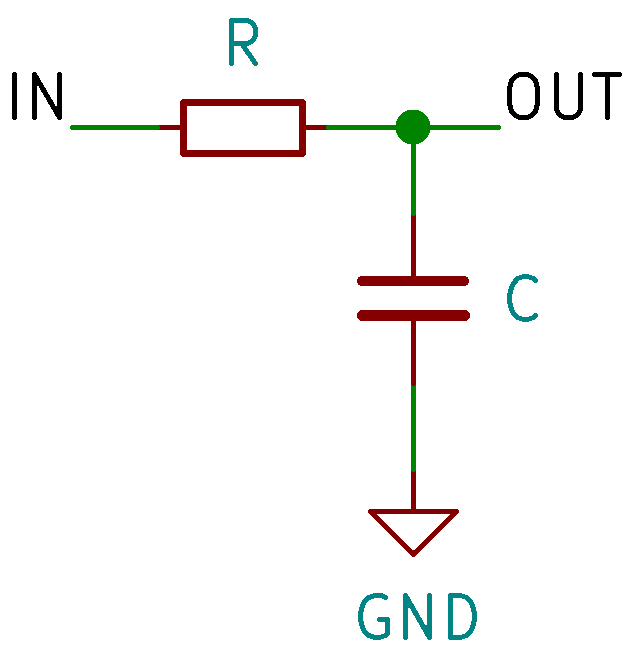
\includegraphics[width=0.2\textwidth]{rc_filter_circuit}
	\caption{The low-pass RC filter used to attenuate high frequency noise.}
	\label{fig:filter}
\end{figure}

A drawback of this filter is that the output voltage is $V_{in} \sqrt{2}$, however it is required due to the type of ADC.
In this case, the maximum voltage the filter can output is $\SI{3.54}{\volt}$.
To acheive maximum output of $\SI{5}{\volt}$, the gain of the amplifier stage would need to be $141$ and the voltage would need to have a $\pm\SI{3.54}{\volt}$ range, centered around $\SI{2.5}{\volt}$.
Due to the requirements, this is not possible as the output voltage of the amplifier saturates at the supply rail voltage.

\subsubsection{Sampling Stage}

The sampling is done using a 12-bit successive approximation (SAR) ADC on the microcontroller.
The SAR hardware is accurate up to high resolutions but requires a stable input, hence the need for an RC filter.
All 12 ADCs exist as different channels on the same ADC peripheral and direct memory acccess (DMA) can be used to move the data to memory.
The ADC peripheral features a hardware averaging circuit which can be leveraged to reduce the load on the microcontroller core.


